\chapter{iSketchNFill: Interactive Sketch \& Fill: Multiclass Sketch-to-Image Translation}

\begin{abstract}
	We propose an interactive GAN-based sketch-to-image translation method that helps novice users create images of simple objects.
	As the user starts to draw a sketch of a desired object type, the network interactively recommends plausible completions, and shows a corresponding synthesized image to the user. This enables a feedback loop, where the user can edit their sketch based on the network's recommendations, visualizing both the completed shape and final rendered image while they draw.
	In order to use a single trained model across a wide array of object classes, we introduce a gating-based approach for class conditioning, which allows us to generate distinct classes without feature mixing, from a single generator network. 
\end{abstract}

\section{Introduction}
Conditional GAN-based image translation \cite{isola2016image2image,sangkloy2017scribbler,zhu2017unpaired} models have shown remarkable success at taking an abstract input, such as an edge map or a semantic segmentation map, and translating it to a real image. Combining this with a user interface allows a user to quickly create images in the target domain. 
However, such interfaces for object creation require the entire edge or label map as input, which is a challenging task as users typically create drawings \emph{incrementally}.
Furthermore, completing a line drawing without any feedback may prove difficult for many, as untrained practitioners generally struggle at free-hand drawing of accurate proportions of objects and their parts~\cite{cohen1997can}, 3D shapes and perspective~\cite{schmidt2009expert}. 
As a result, it is much easier with current interactive image translation methods to obtain realistic looking images by editing \emph{existing} images~\cite{dekel2018sparse,portenier2018faceshop} rather than creating images from scratch. 

We propose a new GAN-based interactive image generation system for drawing objects from scratch that: 1) generates full images given {\em partial} user strokes (or sketches); 2) serves as a \emph{recommender system} that suggests or helps the user \emph{during} their creative process to help them generate a desired image; and 3) uses a single conditional GAN model for {\em multiple} image classes, via a gating-based conditioning mechanism. Such a system allows for creative input to come from the user, while the challenging task of getting exact object proportions correct is left to the model, which constantly predicts a plausible completion of the user's sketch (\figref{fig:teaser}). 

Unlike other related work, we use sparse object outlines/sketches/simplified-edges instead of dense edge maps as the user input
as these are closer to the lines that novice users tend to draw~\cite{cole2008people}. 
Our model first completes the user input and then generates an image conditioned on the completed shape. There are several advantages to this two-stage approach.
For one, we are able to give the artist feedback on the general object shape in our interactive interface (similar to ShadowDraw~\cite{lee2011shadowdraw}), allowing them to quickly refine higher level shape until it is satisfactory.
Second, we found that splitting completion and image generation to work better than going directly from partial outlines to images, as the additional intermediate supervision on full outlines/sketches breaks the problem into two easier sub-problems -- first recover the geometric properties of the object (shape, proportions) and then fill in the appearance (colors, textures). 


For the second stage, we use a multi-class generator that is conditioned on a user supplied class label. This generator applies a gating mechanism that allows the network to focus on the important parts (activations) of the network specific to a given class. Such an approach allows for a clean separation of classes, enabling us to train a single generator and discriminator across \emph{multiple} object classes, thereby enabling a finite-size deployable model that can be used in multiple different scenarios. %based on this gating conditioning.

To demonstrate the potential of our method as an interactive tool for stroke-based image generation, we collect a new image dataset of ten simple object classes (pineapple, soccer, basketball, etc.) with white backgrounds. In order to stress test our conditional generation mechanism, six of the object classes have similar round shapes, which requires the network to derive texture information from the class conditioning. \figref{fig:gui} shows a short video of an interactive editing session using our system. Along with these simple objects, we also demonstrate the potential of our method on more complicated shapes, such as faces and shoes. Code and other details are available at our \href{https://arnabgho.github.io/iSketchNFill/}{website}.



\begin{figure}[t]
	\centering  
	\begin{tabular}{cc}
		%\includegraphics[width=.45\linewidth]{paper_images/isf_method_v3.pdf} &
		\includegraphics[width=.45\linewidth]{images/gif/00001.jpg} \hspace{4pt}
		\includegraphics[width=.45\linewidth]{images/gif_shadow/00001.jpg} 
		%\animategraphics[autoplay,loop,width=.45\linewidth]{25}{images/gif/}{00001}{00266} &
		%\animategraphics[autoplay,loop,width=.50\linewidth]{25}{images/gif_shadow/}{00001}{00096}
		\\
		% (a) & (b) \\
	\end{tabular}
	\caption{{\bf Video of our interface} We can see two versions of our interface. The left side shows how a user can quickly generate multiple objects using a few strokes, while the right side shows the utility of multimodal completions where the user can quickly explore different possible shape generations while drawing. Full video available at our \href{https://arnabgho.github.io/iSketchNFill/}{website}. { \textbf{Please view with Acrobat Reader.}}}\label{fig:gui}
	%\label{fig:gui}}
\end{figure}


\section{Related Work}

\paragraph{Interactive Generation} Interactive interfaces for freehand drawing go all the way back to Ivan Sutherland's Sketchpad~\cite{sutherland64}.  The pre-deep work most related to us, ShadowDraw~\cite{lee2011shadowdraw}, introduced the concept of generating multiple shadows for novice users to be able to draw sketches. PhotoSketcher \cite{eitz2011photosketcher} introduces a retrieval based method for obtaining real images from sketches. %Hays et al.~\cite{hays2007scene} introduce a retrieval-based method for filling scenes.
% \es{other old papers? Talk about ShadowDraw and other non-deep methods}. 
More recently, deep recurrent networks have been used to generate sketches~\cite{ha2017neural,ganin2018synthesizing}. Sketch-RNN~\cite{ha2017neural} provides a completion of partial strokes, with the advantage of intermediate stroke information via the Quickdraw dataset at training time. SPIRAL \cite{ganin2018synthesizing} learns to generate digits and faces using a reinforcement learning approach.
% to generate programs for synthesizing the final image.
Zhu et al.~\cite{zhu2016generative} train a generative model, and an optimization-based interface to generate possible images, given color or edge constraints. The technique is limited to a single class and does not propose a recommendation for the completion of the shape. SketchyGAN~\cite{chen2018sketchygan} also aimed at generating multi-class images but lacks interactive capability. In contrast to the above, our method provides interactive prediction of the shape and appearance to the user and supports multiple object classes.
% \vspace{-6mm}
\paragraph{Generative Modeling} Parametric modeling of an image distribution is a challenging problem. Classic approaches include autoencoders~\cite{hinton2006reducing,vincent2008extracting} and Boltzmann machines~\cite{smolensky1986information}. More modern approaches include autoregressive models~\cite{efros1999texture,van2016conditional}, variational autoencoders (VAEs)~\cite{kingma2013auto}, and generative adversarial networks (GANs). GANs and VAEs both learn mappings from a low-dimensional ``latent" code, sampled stochastically, to a high-dimensional image through a feedforward pass of a network. GANs have been successful recently~\cite{denton2015deep,radford2015unsupervised,arjovsky2017wgan}, and hybrid models feature both a learned mapping from image to latent space as well as adversarial training~\cite{donahue2016adversarial,dumoulin2016adversarially,larsen2016vaegan,chen2016infogan}.

% \vspace{2mm} 
\paragraph{Conditioned Image Generation} The methods described above can be conditioned, either by a low-dimensional vector (such as an object class, or noise vector), a high-dimensional image, or both. Isola et al.~\cite{isola2016image2image} propose ``pix2pix", establishing the general usefulness of conditional GANs for image-to-image translation tasks. However, they discover that obtaining multimodality by injecting a random noise vector is difficult, a result corroborated in~\cite{mathieu2015deep,pathak2016context,zhu2017toward}.
% introduced a set of tasks whereby the pixels of the input in a different domain corresponded to the pixels of the generated image.
% As a result, image-to-image translation methods have exploded in popularity, as many applications can be expressed in this framework.
% However, one problem with the original Pix2pix formulation is that the quality degrades quickly with increased class diversity. 
% We build upon these ideas by proposing a new architecture and gating scheme that allows for high quality multiclass image generation. 
% \paragraph{Mode Collapse}
This is an example of mode collapse~\cite{goodfellow2016nips}, a phenomenon especially prevalent in image-to-image GANs, as the generator tends or ignore the low-dimensional latent code in favor of the high-dimensional image.
% This is an example of mode collapse is a major challenge for GANs~\cite{goodfellow2016nips}, where the diversity of the generated results is limited and only a portion of the training set is utilized. 
Proposed solutions include layers which better condition the optimization, such as Spectral Normalization~\cite{zhang2018self,miyato2018spectral}, modifications to the loss function, such as WGAN~\cite{arjovsky2017wasserstein,gulrajani2017improved} or optimization procedure~\cite{heusel2017gans}, or modeling proposals, such as MAD-GAN~\cite{ghosh2017multi} and MUNIT~\cite{huang2018multimodal}. 
% Several techniques deal with this issue, the best performing among those include Spectral Normalization \cite{zhang2018self,miyato2018spectral} which normalizes the spectral norms of the layers to stabilize training, MAD-GAN \cite{ghosh2017multi} which introduces multiple generators, BicycleGAN \cite{zhu2017toward} which reconstructs the latent code from the generation using two cycles, and MUNIT \cite{huang2018multimodal} which introduces a factorized latent space for content and style for producing variations.
One modeling approach is to add a predictor from the output to the conditioner, to discourage the model from ignoring the conditioner. This has been explored in the classification setting in Auxiliary-Classifier GAN (ACGAN)~\cite{odena2016conditional} and regression setting with InfoGAN~\cite{chen2016infogan} and ALI/BiGAN (``latent regressor" model)~\cite{dumoulin2016adversarially,donahue2016adversarial}, and is one half of BicycleGAN model~\cite{zhu2017toward}. We explore a complementary approach of architectural modification via gating.


\noindent \textbf{Gating Mechanisms}
%Residual Networks \cite{he2016deep} introduced a new set of architectures that enabled training of very deep networks.
Residual networks~\cite{he2016deep}, first introduced for image classification~\cite{krizhevsky2012imagenet}, have made extremely deep networks viable to train. Veit et al.~\cite{veit2016residual} find that the skip connection in the architecture enables test-time removal of blocks. Follow-up work~\cite{veit2018adaptive} builds in block removal during training time, with the goal of subsets of blocks specializing to different categories. Inspired by these results, we propose the use of gating for image generation and provide a systematic analysis of gating mechanisms.
% Prior work has demonstrated that in ResNets, some paths are more important for particular classes~\cite{veit2016residual}, and has used this to develop a hard gating mechanism~\cite{veit2018adaptive}.
% We provide a further analysis of gating mechanisms, in the context of GAN image generation, as opposed to image classification.

The adaptive instance normalization (AdaIn) layer has similarly been used in arbitrary style transfer~\cite{huang2017arbitrary} and image-to-image translation~\cite{huang2018multimodal}, and Feature-wise Linear Modulation (FiLM)~\cite{perez2017film}. Both methods scale and shift feature distributions, based on a high-dimensional conditioner, such as an image or natural language question. Gating also plays an important role in sequential models for natural language processing: LSTMs \cite{hochreiter1997long} and GRU \cite{cho2014learning}. Similarly, concurrent work \cite{karras2018style}, \cite{park2019semantic} use a AdaIN-style network to modulate the generator parameters.
% \es{Mention concurrent work? StyleGAN, Taesung's paper}


\begin{figure}[t]
	\centering  
	% \begin{tabular}{cc}
	\includegraphics[width=\linewidth]{paper_images/isf_method_v3.pdf} 
	% \includegraphics[width=.55\linewidth]{paper_images/shapegen.pdf}
	\\
	% (a) & (b) \\
	% \end{tabular}
	\vspace{-4mm}
	\caption{{\bf Our two-stage approach} First, we complete a partial sketch using the shape generator $G_S$. Then we translate the completed sketch into an image using the appearance generator $G_A$. Both generators are trained with their respective discriminators $D_S$, and $D_A$.
		{}}\label{fig:SketchFillNet}
	%\label{fig:gui}}
\end{figure}




\begin{figure*}[t]
	\centering
	% \includegraphics[width=\linewidth]{images/shape_completion/shape_completion.pdf}
	\includegraphics[width=\linewidth]{paper_images/shapegen.pdf}
	\vspace{-8mm}
	\caption{\textbf{First stage (Shape Generator)} To achieve multi-modal completions, the shape generator is designed using inspiration from non-image conditional model \cite{mescheder2018training} with the conditioning input provided at multiple scales, so that the generator network doesn't ignore the partial stroke conditioning.
		%$G_S$ design inspired from unconditional generator, with the conditioning provided at multiple scales to $G_S$ and $D_S$
	}\label{fig:SketchNet}
	%\vspace{-2mm}
\end{figure*}

\label{sec:methods}

\vspace{-4mm}
\section{Method}
We decouple the problem of interactive image generation into two stages: object shape completion from sparse user sketches, and appearance synthesis from the completed shape. More specifically, as illustrated in \figref{fig:SketchFillNet} we use the Shape Generator $G_S$ for the automatic shape (outline/sparse-sketch/simplified-edge) generation and the Appearance Generator $G_A$ for generating the final image as well as the adversary discriminators $D_S$ and $D_A$. Example usage is shown in our user interface in \figref{fig:gui}.

\subsection{Shape completion}
\label{sec:shape}
The shape completion network $G_S$ should provide the user with a visualization of its completed shape(s), based on the user input, and should keep on updating the suggested shape(s) interactively. 
%For an interactive user interface to be effective, the network has to generate an estimated full image shape as the user adds sparse input. 
We take a data-driven approach for this whereby, to train the network, we simulate partial strokes (or inputs) by removing random square patches from the full outline/ full sparse sketch/ full simplified edges. 
The patches are of three sizes (64$\times$64, 128$\times$128, 192$\times$192) and placed at a random location in the image of size 256$\times$256 (see \figref{fig:autocomplete_data_generation} for an example). To extend the technique beyond outlines and generate more human-like sketches, we adopt the multistage procedure depicted in \figref{fig:simplified_edges}. We refer to these generated sketches as ``simplified edges''.
% \es{probably need more details here - size of squares, how many per image, total training data size etc.}
We automatically generate data in this manner, creating a dataset where for a given full outline/sketch or a simplified edge-map, 75 different inputs are created.
%We found that the BicycleGAN model~\cite{zhu2017toward} performed well on the shape completion task, and we train it, unmodified, on pairs of partial-full outline images. %(Fig.~\ref{fig:infogan_gate}, top left).
The model, shown in \figref{fig:SketchFillNet}, is based on the architecture used for non-image conditional generations in \cite{mescheder2018training}. We modify the architecture such that the conditioning input is provided to the generator and discriminator at multiple scales as shown in \figref{fig:SketchNet}. This makes the conditioning input an active part of the generation process and helps in producing multimodal completions.


\begin{figure}[t]
	\centering
	\begin{tabular}{*{4}{c@{\hspace{3px}}}}
		\frame{\includegraphics[width=.22\linewidth]{images/autocomplete_data_generation/original.png}} &
		\frame{\includegraphics[width=.22\linewidth]{images/autocomplete_data_generation/64.png}} &
		\frame{\includegraphics[width=.22\linewidth]{images/autocomplete_data_generation/128.png}} &
		\frame{\includegraphics[width=.22\linewidth]{images/autocomplete_data_generation/192.png}}\\
		Outline &
		% 64$\times$64&
		% 128$\times$128 &
		% 192$\times$192
		\multicolumn{3}{c}{Simulated Partial Inputs}
		\\
	\end{tabular} \\
	\vspace{-3mm}
	\caption{\textbf{Simulated Inputs} Three sizes of occluders were used to simulate partial outlines.}
	\label{fig:autocomplete_data_generation}
\end{figure}

\begin{figure}[t]%[ht!]
	\centering
	\begin{tabular}{*{4}{c@{\hspace{3px}}}}
		\frame{\includegraphics[width=.22\linewidth]{images/edge_simplification/1.jpg}} &
		\frame{\includegraphics[width=.22\linewidth]{images/edge_simplification/1_edge.jpg}} &
		\frame{\includegraphics[width=.22\linewidth]{images/edge_simplification/1_edge_tone.jpg}} &
		\frame{\includegraphics[width=.22\linewidth]{images/edge_simplification/1_simplified_edge.jpg}}
		\\
		
		% \begin{subfigure}[t]{.25\linewidth}\caption{}\label{fig:basketball_partial}\end{subfigure} &
		% \begin{subfigure}[t]{.25\linewidth}\caption{}\label{fig:basketball_full}\end{subfigure} &
		% \begin{subfigure}[t]{.25\linewidth}\caption{}\label{fig:basketball_full}\end{subfigure} &
		% \begin{subfigure}[t]{.25\linewidth}\caption{}\label{fig:soccer_partial}\end{subfigure} \\
	\end{tabular} \\
	\caption{\textbf{Simplified Edges} The 2nd edgemap is obtained using the technique of \cite{isola2016image2image}, while the 3rd is the intermediate edgemap using \cite{li2019im2pencil} and further simplified using \cite{simo2016learning} which looks closer to what a human would sketch. }
	\label{fig:simplified_edges}
	\vspace{-3mm}
\end{figure}

\vspace{-4mm}
\begin{figure*}[t]
	\centering
	\includegraphics[width=1.\linewidth]{paper_images/arch_inject2.pdf}
	\vspace{-6mm}
	\caption{
		% \vspace{-2mm}
		{\bf Conditioning variants for the Appearance Generator} Our model uses gating on all the residual blocks of the generator and the discriminator, other forms of conditioning such as (naive concatenation in input only, all layers, AC-GAN like latent regressor \cite{odena2016conditional}) are evaluated as well. \label{fig:arch-gate1}
		% \vspace{-2mm}
	}
\end{figure*}

\begin{figure*}[t]
	\centering
	\includegraphics[width=1.\linewidth]{paper_images/arch_gate3.pdf}
	\vspace{-4mm}
	\caption{
		% {\bf Incorporating soft-gating into residual blocks.} \rz{Order got changed, may or may not need to add key for hadamard product}
		{\bf Injecting conditioning with modified residual layers} {\bf (Left)} A ``vanilla" residual block without conditioning applies a residual modification to the input tensor. {\bf (Mid-left)} The $\mathcal{H}(X)$ block is softly-gated by scalar parameter $\alpha$ and shift $\beta$. {\bf (Mid)} Adaptive Instance Normalization~\cite{huang2017arbitrary} applies a channel-wise scaling and shifting after an instance normalization layer. {\bf (Mid-right)} Channel-wise gating adds restrictions to the range of $\mbox{\boldmath $\alpha$}$. {\bf (Right)} We find that channel-wise gating (without added bias) produces the best results empirically.\label{fig:arch-gate2}
		\vspace{-2mm}
	}
\end{figure*}


\vspace{4mm}
\subsection{Appearance synthesis}
\label{sec:appearance}
%We use a conditional GAN formulation for generating images from outlines as shown by the efficacy in \cite{isola2016image2image,zhu2017toward}. 
An ideal interactive sketch-to-image system  should be able to generate multiple different image classes with a single generator. 
Beside memory and time considerations (avoiding loading/using a separate model per class, reducing overall memory), a single network can share features related to outline recognition and texture generation that are common across classes, which helps training with limited examples per class. %\es{Didn't we already said that in the intro? If yes we should remove/significantly shorten}

As we later show, class-conditioning by concatenation can fail to properly condition the network about the class information in current image translation networks~\cite{isola2016image2image,zhu2017toward}.
%
To address this, we propose an effective soft gating mechanism, shown in~\figref{fig:arch-gate1}.
Conceptually, our network consists of a small external gating network that is conditioned on the object class (encoded as a 1-hot vector).
The gating network outputs parameters that are used to modify the features of the main generator network.
Given an input feature tensor $X_l$, ``vanilla'' ResNet~\cite{he2016deep} maps it to
\begin{equation}
	X_{l+1} = X_l+\mathcal{H}_l(X_l).
\end{equation}
Changes in resolution are obtained by upsampling before or downsampling after the residual block.
Note that we omit $l$ subscript from this point forward to reduce clutter.
Our gating network augments this with a predicted scalar $\alpha$ for each layer of the network using a learned network $\mathcal{F}({\bf y})$, where ${\bf y}$ is the conditioning vector:
\begin{equation}
	X + \alpha \; \mathcal{H}(X), \text{where } \alpha \in [0,1]
\end{equation}

If the conditioning vector ${\bf y}$ has no use for a particular block, it can predict $\alpha$ close to zero and effectively switch off the layer.
% , and use that layer instead for other classes.
During training, blocks within the main network can transform the image in various ways, and $\mathcal{F}$ can modulate such that the most useful blocks are selected. 
Unlike previous feature map conditioning methods such as AdaIn~\cite{ulyanovinstance}, we apply gating to \emph{both} the generator and discriminator. 
This enables the discriminator to select blocks which effectively judge whether generations are real or fake, conditioned on the class input.
% Via accurate gradients backpropagated to the generator it also enables the generator to generate class conditioned high resolution image samples.
Some blocks can be shared across regions in the conditioning vector, whereas other blocks can specialize for a given class.

A more powerful method is to apply this weighting channel-wise using a vector {\boldmath$\alpha$}: % This is denoted as follows:
\begin{align}
	X + \mbox{\boldmath $\alpha$} \odot \mathcal{H}(X), \text{where } \mbox{\boldmath $\alpha$} \in [0,1]^c, 
\end{align}
where $\odot$ represents channel-wise multiplication. This allows specific channels to be switched ``on" or ``off", providing additional degrees of freedom.
%We make the corresponding changes in the discriminator as well. 
%Soft-gating has been explored by Veit et al.~\cite{veit2018adaptive} in a classification setting. 
We found that this channelwise approach for gating provides the strongest results. 
AdaIn describes the case where an Instance Normalization~\cite{ulyanovinstance} (IN) operation is applied before scaling and shifting the feature distribution.
We constrain each element of {\boldmath $\alpha$} and {\boldmath $\beta$} in $[-1, 1]$.
We additionally explored incorporating a bias term after the soft-gating, either block-wise using a scalar $\beta \in [-1,1]$ per layer, or channel-wise using a vector $\mbox{\boldmath $\beta$} \in [-1, 1]^c$ per layer but we found that they did not help much, and so we leave them out of our final model. Refer \figref{fig:arch-gate2} for pictorial representation of various gatings.
% \ow{but found that they did not help much, and so we leave them out of our final model?}


Finally, we describe our network architecture, which utilizes the gated residual blocks described above.
We base our architecture on the proposed residual \textbf{Encoder-Decoder} model from MUNIT~\cite{huang2018multimodal}.
This architecture is comprised of 3 \texttt{conv} layers, 8 residual blocks, and 3 \texttt{up-conv} layers. The residual blocks have 256 channels. 
First, we deepen the network, based on the principle that deeper networks have more valid disjoint, partially shared paths~\cite{veit2016residual}, and add 24 residual blocks. 
To enable the larger number of residual blocks, we drastically reduce the width to 32 channels for every layer. 
We refer to this network as \textbf{SkinnyResNet}. 
Additionally, we found that modifying the downsampling and upsampling blocks to be residual connections as well improved results, and also enables us to apply gating to {\em all} blocks. 
When gating is used, the gate prediction network, $\mathcal{F} ({\bf y})$,  
%Fig.~\ref{fig:arch-inj} (mid-right, right) 
is also designed using residual blocks. Additional architecture details are in the supplementary material. 


\begin{figure*}[t]
	\begin{tabular}{cc}
		\resizebox{0.5\linewidth}{!}{
			\begin{tabular}{*{5}{c@{\hspace{3px}}}}
				\frame{\includegraphics[width=.12\linewidth]{images/shoe_autocomplete_render/current_scribble_5.jpg}} &
				%\frame{\includegraphics[width=.10\linewidth]{images/autocomplete_generate/scribble/soccer.png}} &
				\frame{\includegraphics[width=.12\linewidth]{images/shoe_autocomplete_render/current_scribble_6.jpg}} & 
				\frame{\includegraphics[width=.12\linewidth]{images/shoe_autocomplete_render/current_scribble_7.jpg}}&
				\frame{\includegraphics[width=.12\linewidth]{images/shoe_autocomplete_render/current_scribble_8.jpg}} &
				\\
				\frame{\includegraphics[width=.12\linewidth]{images/shoe_autocomplete_render/autocompleted_sketch_5.png}} &
				%\frame{\includegraphics[width=.10\linewidth]{images/autocomplete_generate/scribble/soccer.png}} &
				\frame{\includegraphics[width=.12\linewidth]{images/shoe_autocomplete_render/autocompleted_sketch_6.png}} & 
				\frame{\includegraphics[width=.12\linewidth]{images/shoe_autocomplete_render/autocompleted_sketch_7.png}}&
				\frame{\includegraphics[width=.12\linewidth]{images/shoe_autocomplete_render/autocompleted_sketch_8.png}} &
				
				\\
				\frame{\includegraphics[width=.12\linewidth]{images/shoe_autocomplete_render/rendered_5.png}} &
				%\frame{\includegraphics[width=.10\linewidth]{images/autocomplete_generate/scribble/soccer.png}} &
				\frame{\includegraphics[width=.12\linewidth]{images/shoe_autocomplete_render/rendered_6.png}} & 
				\frame{\includegraphics[width=.12\linewidth]{images/shoe_autocomplete_render/rendered_7.png}}&
				\frame{\includegraphics[width=.12\linewidth]{images/shoe_autocomplete_render/rendered_8.png}} &
				
				\\
			\end{tabular}
		}
		& 
		\resizebox{0.5\linewidth}{!}{
			\begin{tabular}{*{5}{c@{\hspace{3px}}}}
				\frame{\includegraphics[width=.12\linewidth]{images/face_autocomplete_render/current_scribble_6.jpg}} &
				%\frame{\includegraphics[width=.10\linewidth]{images/autocomplete_generate/scribble/soccer.png}} &
				\frame{\includegraphics[width=.12\linewidth]{images/face_autocomplete_render/current_scribble_7.jpg}} & 
				\frame{\includegraphics[width=.12\linewidth]{images/face_autocomplete_render/current_scribble_8.jpg}}&
				\frame{\includegraphics[width=.12\linewidth]{images/face_autocomplete_render/current_scribble_9.jpg}} &
				\\
				\frame{\includegraphics[width=.12\linewidth]{images/face_autocomplete_render/autocompleted_sketch_6.png}} &
				%\frame{\includegraphics[width=.10\linewidth]{images/autocomplete_generate/scribble/soccer.png}} &
				\frame{\includegraphics[width=.12\linewidth]{images/face_autocomplete_render/autocompleted_sketch_7.png}} & 
				\frame{\includegraphics[width=.12\linewidth]{images/face_autocomplete_render/autocompleted_sketch_8.png}}&
				\frame{\includegraphics[width=.12\linewidth]{images/face_autocomplete_render/autocompleted_sketch_9.png}} &
				
				\\
				\frame{\includegraphics[width=.12\linewidth]{images/face_autocomplete_render/rendered_6.png}} &
				%\frame{\includegraphics[width=.10\linewidth]{images/autocomplete_generate/scribble/soccer.png}} &
				\frame{\includegraphics[width=.12\linewidth]{images/face_autocomplete_render/rendered_7.png}} & 
				\frame{\includegraphics[width=.12\linewidth]{images/face_autocomplete_render/rendered_8.png}}&
				\frame{\includegraphics[width=.12\linewidth]{images/face_autocomplete_render/rendered_9.png}} &
				
				\\
			\end{tabular}
		} 
		
	\end{tabular}
	\vspace{-2mm}
	\caption{\textbf{Example Sketch \& Fill Progression.} The \textbf{first row} represents the progressive addition of new strokes on the canvas, the \textbf{second row} shows the autocompleted sketch, and the \textbf{third row} is the final generated image. 
		As the sparse strokes are changed by the user, the completed shape and generated image evolve as well. Note that changing a stroke locally produces coherent changes in other parts of the image.
		\vspace{-4mm}
	}
	% \es{replace orange and chicken. maybe also moon and cupcake.}}
	\label{fig:autocomplete_generate_sketches}
\end{figure*}

\begin{figure*}[t]
	\centering
	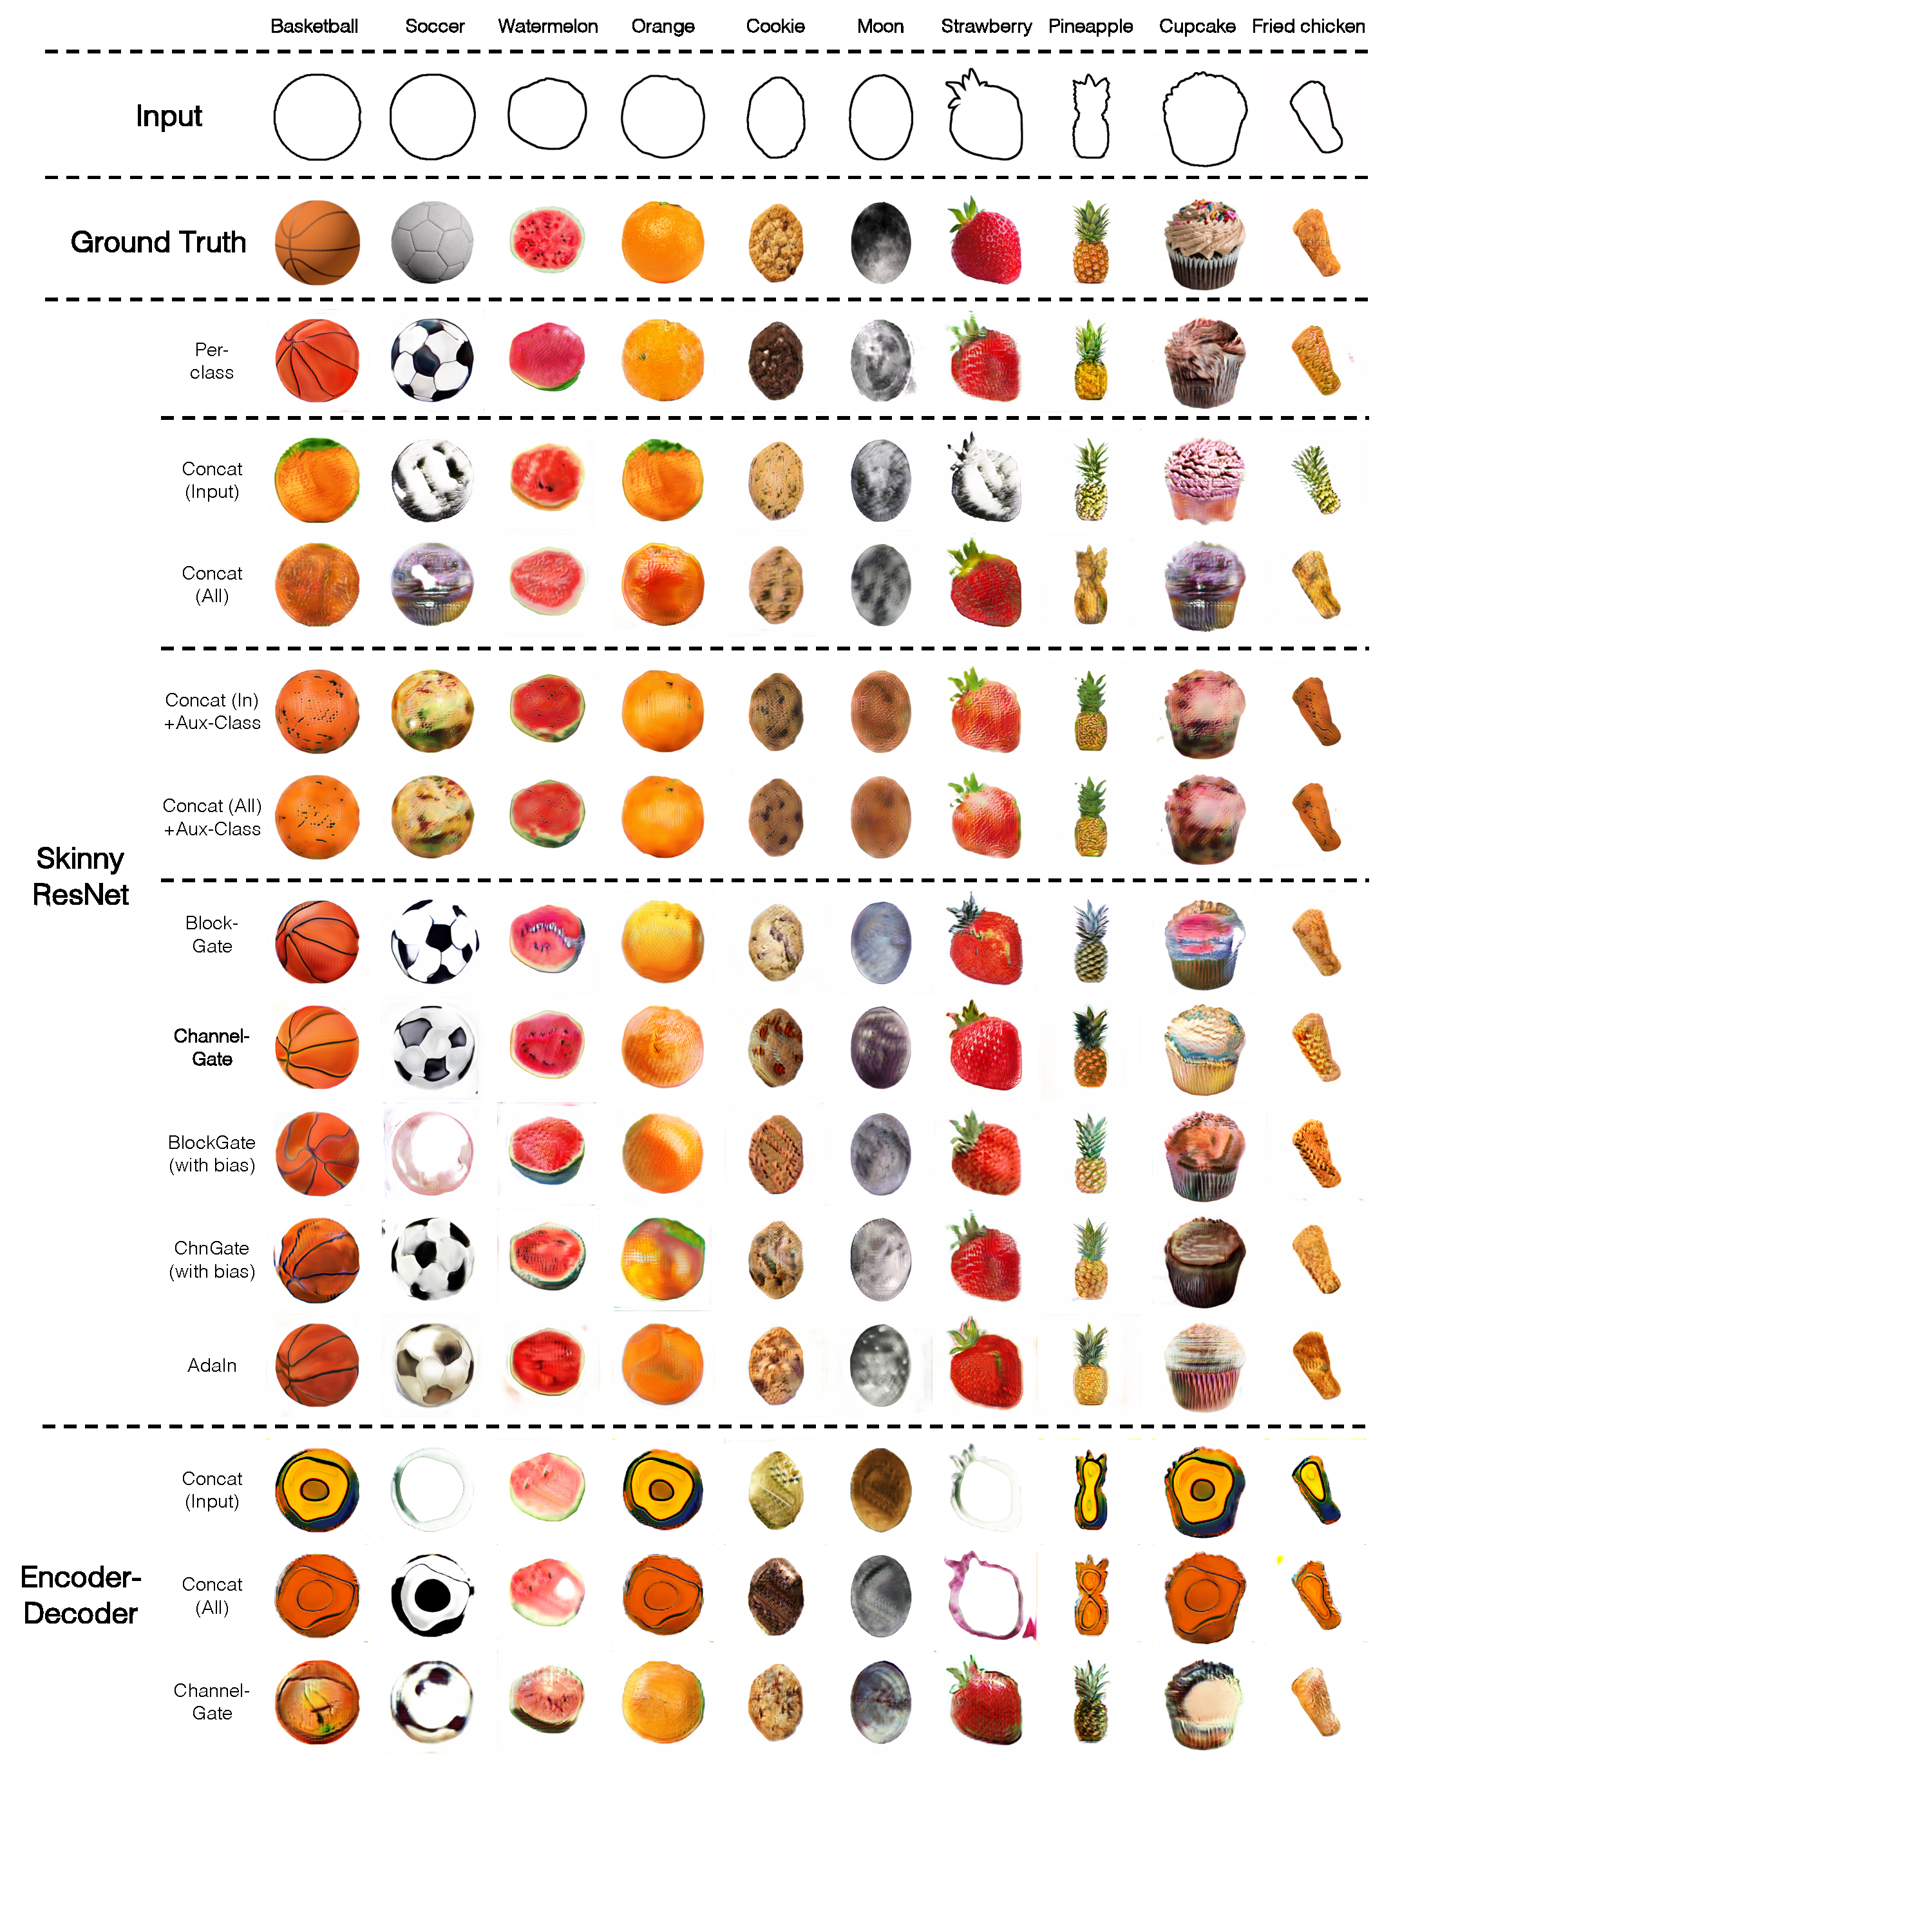
\includegraphics[width=.9\linewidth]{paper_images/cond_comp2.pdf}
	\caption{{\bf Conditioning injection comparison.} We show results across methods on the outline$\rightarrow$image task using the \textbf{SkinnyResNet} architecture. Naive Concatenation \textbf{Concat} often confuses classes, such as oranges and basketballs, while gating mechanisms such as the \textbf{ChannelGate} method succeed. The gating method also improves results for the \textbf{EncoderDecoder} architecture. \label{fig:alg_comp} }
	\vspace{-4mm}
\end{figure*}

\vspace{-4mm}
\section{Experiments}
\label{sec:experiments}
We first compare our 2 step approach for interactive image generation on existing datasets such as the UTZappos Shoes dataset \cite{yu2014fine} and CelebA-HQ \cite{karras2017progressive}. State-of-the-art techniques such as pix2pixHD \cite{Wang_2018_CVPR} are used to generate the final image from the autocompleted sketches. We finally evaluate our approach on a multi-class dataset that we collected to test our proposed gating mechanism.


\begin{table}[t]
	\resizebox{1.\linewidth}{!} {
		\centering
		\begin{tabular}{l c}
			% \hline
			\toprule
			\textbf{Trained task} & \textbf{FID} \\ \midrule
			% PE $\rightarrow$ Image & 73.12 \% \\
			% PO $\rightarrow$ Image & 88.74 \% \\
			% EC $\rightarrow$ FE $\rightarrow$ Image & 45.96 \% \\
			% OC $\rightarrow$ FO $\rightarrow$ Image \textbf{[Ours]} & \textbf{97.38\%}  \\
			\textbf{Faces}\\ \hline
			Partial Simplified Edges $\rightarrow$ Image & 383.02 \\
			Partial Simplified Edges $\rightarrow$ Simplified Edges $\rightarrow$ Image & 374.67 \\
			\hline
			\textbf{Shoes}\\ \hline
			Partial Simplified Edges $\rightarrow$ Image & 170.45 \\
			Partial Simplified Edges $\rightarrow$ Simplified Edges $\rightarrow$ Image & 154.32 \\
			% Partial edges $\rightarrow$ Full edges $\rightarrow$ Image & 45.96 \% \\
			% \cdashline{1-2}
			% Partial outline $\rightarrow$ Full outline $\rightarrow$ Image [Ours] & \textbf{97.38\%}  \\
			\bottomrule %inserts single line
		\end{tabular}
	}
	\vspace{-2mm}
	\caption{\label{table:2step_eval_single_class} \textbf{Single-class generation, 2-stage vs 1-stage}. We evaluate the result quality from different task pipelines.
		% Evaluates the result quality from different trained task pipelines, including Partial Edges (PE), Partial Outlines (PO), Edge Completion (EC), Full Edges (FE), Outline Completion (OC), and Full Outlines (FO). Accuracy is computed by a fixed, pretrained classification network, on the resulting images.
		\vspace{-4mm}
	}
\end{table}
\vspace{-2mm}
\subsection{Single Class Generation}
\paragraph{Datasets} We use the edges2shoes\cite{isola2016image2image}, CelebA-HQ\cite{karras2017progressive} datasets to test our method on single class generation. 
We simplify the edges to attempt to more closely resemble how humans would draw strokes by first using the preprocessing code of \cite{li2019im2pencil} further reducing the strokes with a sketch simplification network \cite{simo2016learning}.
\paragraph{Architecture} We use the architecture described in Section \ref{sec:shape} for shape completion. In this case, each dataset only contains a single class, so we can use an off-the-shelf network, such as pix2pixHD~\cite{wang2017high} for rendering.

\paragraph{Results} As seen in \figref{fig:autocomplete_generate_sketches}, our 2 step technique allows us to complete the simplified edge maps from the partial strokes and also generate realistic images from the autocompleted simplified edges.
Table \ref{table:2step_eval_single_class} also demonstrates, across two datasets (faces and shoes), that using a 2 step procedure produces stronger results than mapping directly from the partial sketch to the completed image.

\begin{table}[t]
	\centering
	\begin{tabular}{l c}
		% \hline
		\toprule
		\textbf{Trained task} & \textbf{Avg Acc} \\ \midrule
		% PE $\rightarrow$ Image & 73.12 \% \\
		% PO $\rightarrow$ Image & 88.74 \% \\
		% EC $\rightarrow$ FE $\rightarrow$ Image & 45.96 \% \\
		% OC $\rightarrow$ FO $\rightarrow$ Image \textbf{[Ours]} & \textbf{97.38\%}  \\
		Partial edges $\rightarrow$ Image & 73.12 \% \\
		Partial outline $\rightarrow$ Image & 88.74 \% \\
		% Partial edges $\rightarrow$ Full edges $\rightarrow$ Image & 45.96 \% \\
		% \cdashline{1-2}
		Partial outline $\rightarrow$ Full outline $\rightarrow$ Image [Ours] & \textbf{97.38\%}  \\
		\bottomrule %inserts single line
	\end{tabular}
	\vspace{-2mm}
	\caption{\label{table:2step_eval} \textbf{Multi-class generation, 2-stage vs 1-stage}. We evaluate the result quality from different task pipelines. Accuracy is computed by a fixed, pretrained classification network, on the resulting images.
		% Evaluates the result quality from different trained task pipelines, including Partial Edges (PE), Partial Outlines (PO), Edge Completion (EC), Full Edges (FE), Outline Completion (OC), and Full Outlines (FO). Accuracy is computed by a fixed, pretrained classification network, on the resulting images.
		\vspace{-1mm}
	}
\end{table}




\begin{figure}[t]%[ht!]
	\centering
	\begin{tabular}{*{6}{c@{\hspace{3px}}}}
		\frame{\includegraphics[width=.15\linewidth]{images/ablation_images/basketball_partial_outline.png}} &
		\frame{\includegraphics[width=.15\linewidth]{images/ablation_images/basketball_full_outline.png}} &
		\frame{\includegraphics[width=.15\linewidth]{images/ablation_images/soccer_partial_outline.png}} & 
		\frame{\includegraphics[width=.15\linewidth]{images/ablation_images/soccer_full_outline.png}}&
		\frame{\includegraphics[width=.15\linewidth]{images/ablation_images/cupcake_partial_outline.png}} &
		\frame{\includegraphics[width=.15\linewidth]{images/ablation_images/cupcake_full_outline.png}}
		\\
		
		\frame{\includegraphics[width=.15\linewidth]{images/ablation_images/basketball_partial_outline_gen.png}} &
		\frame{\includegraphics[width=.15\linewidth]{images/ablation_images/basketball_full_outline_gen.png}} &
		\frame{\includegraphics[width=.15\linewidth]{images/ablation_images/soccer_partial_outline_gen.png}} & 
		\frame{\includegraphics[width=.15\linewidth]{images/ablation_images/soccer_full_outline_gen.png}}&
		\frame{\includegraphics[width=.15\linewidth]{images/ablation_images/cupcake_partial_outline_gen.png}} &
		\frame{\includegraphics[width=.15\linewidth]{images/ablation_images/cupcake_full_outline_gen.png}}
		\\
		
		% \begin{subfigure}[t]{.15\linewidth}\caption{}\label{fig:basketball_partial}\end{subfigure} &
		% \begin{subfigure}[t]{.15\linewidth}\caption{}\label{fig:basketball_full}\end{subfigure} &
		% \begin{subfigure}[t]{.15\linewidth}\caption{}\label{fig:soccer_partial}\end{subfigure} &
		% \begin{subfigure}[t]{.15\linewidth}\caption{}\label{fig:soccer_full}\end{subfigure} &
		% \begin{subfigure}[t]{.15\linewidth}\caption{}\label{fig:cupcake_partial}\end{subfigure} &
		% \begin{subfigure}[t]{.15\linewidth}\caption{}\label{fig:cupcake_full}\end{subfigure}\\
	\end{tabular}
	\caption{\textbf{Directly mapping from partial outline to image} Our proposed system uses a 2-stage approach, using a completed edge map as an intermediate. Here, we show results when directly mapping from the partial outline to the image. When the outline is well-defined, the network can generate realistic images. However, when the outline is sparse, the network struggles with the geometry.}
	\label{fig:ablation_partial_full_outline}
	\vspace{-3mm}
\end{figure}

\begin{figure}[t]%[ht!]
	\centering
	\resizebox{1.0\linewidth}{!}{
		\begin{tabular}{*{5}{c@{\hspace{3px}}}}
			\frame{\includegraphics[width=.2\linewidth]{images/autocomplete_generate/scribble/basketball.png}} &
			%\frame{\includegraphics[width=.10\linewidth]{images/autocomplete_generate/scribble/soccer.png}} &
			\frame{\includegraphics[width=.2\linewidth]{images/autocomplete_generate/scribble/watermelon.png}} & 
			\frame{\includegraphics[width=.2\linewidth]{images/autocomplete_generate/scribble/orange.png}}&
			\frame{\includegraphics[width=.2\linewidth]{images/autocomplete_generate/scribble/cookie.png}} &
			%\frame{\includegraphics[width=.10\linewidth]{images/autocomplete_generate/scribble/moon.png}} &
			%\frame{\includegraphics[width=.10\linewidth]{images/autocomplete_generate/scribble/strawberry.png}} &
			\frame{\includegraphics[width=.2\linewidth]{images/autocomplete_generate/scribble/pineapple.png}}
			%\frame{\includegraphics[width=.10\linewidth]{images/autocomplete_generate/scribble/cupcake.png}} &
			%\frame{\includegraphics[width=.10\linewidth]{images/autocomplete_generate/scribble/chicken.png}}
			\\
			
			\frame{\includegraphics[width=.2\linewidth]{images/autocomplete_generate/autocomplete/basketball.png}} &
			%\frame{\includegraphics[width=.10\linewidth]{images/autocomplete_generate/autocomplete/soccer.png}} &
			\frame{\includegraphics[width=.2\linewidth]{images/autocomplete_generate/autocomplete/watermelon.png}} & 
			\frame{\includegraphics[width=.2\linewidth]{images/autocomplete_generate/autocomplete/orange.png}}&
			\frame{\includegraphics[width=.2\linewidth]{images/autocomplete_generate/autocomplete/cookie.png}} &
			%\frame{\includegraphics[width=.10\linewidth]{images/autocomplete_generate/autocomplete/moon.png}} &
			%\frame{\includegraphics[width=.10\linewidth]{images/autocomplete_generate/autocomplete/strawberry.png}} &
			\frame{\includegraphics[width=.2\linewidth]{images/autocomplete_generate/autocomplete/pineapple.png}}
			%\frame{\includegraphics[width=.10\linewidth]{images/autocomplete_generate/autocomplete/cupcake.png}} &
			%\frame{\includegraphics[width=.10\linewidth]{images/autocomplete_generate/autocomplete/chicken.png}}
			\\
			
			
			\frame{\includegraphics[width=.2\linewidth]{images/autocomplete_generate/image/basketball.png}} &
			%\frame{\includegraphics[width=.10\linewidth]{images/autocomplete_generate/image/soccer.png}} &
			\frame{\includegraphics[width=.2\linewidth]{images/autocomplete_generate/image/watermelon.png}} & 
			\frame{\includegraphics[width=.2\linewidth]{images/autocomplete_generate/image/orange.png}}&
			\frame{\includegraphics[width=.2\linewidth]{images/autocomplete_generate/image/cookie.png}} &
			%\frame{\includegraphics[width=.10\linewidth]{images/autocomplete_generate/image/moon.png}} &
			%\frame{\includegraphics[width=.10\linewidth]{images/autocomplete_generate/image/strawberry.png}} &
			\frame{\includegraphics[width=.2\linewidth]{images/autocomplete_generate/image/pineapple.png}}
			%\frame{\includegraphics[width=.10\linewidth]{images/autocomplete_generate/image/cupcake.png}} &
			%\frame{\includegraphics[width=.10\linewidth]{images/autocomplete_generate/image/chicken.png}}
			\\
			% \begin{subfigure}[t]{.15\linewidth}\caption{}\label{fig:basketball_partial}\end{subfigure} &
			% \begin{subfigure}[t]{.15\linewidth}\caption{}\label{fig:basketball_full}\end{subfigure} &
			% \begin{subfigure}[t]{.15\linewidth}\caption{}\label{fig:soccer_partial}\end{subfigure} &
			% \begin{subfigure}[t]{.15\linewidth}\caption{}\label{fig:soccer_full}\end{subfigure} &
			% \begin{subfigure}[t]{.15\linewidth}\caption{}\label{fig:cupcake_partial}\end{subfigure} &
			% \begin{subfigure}[t]{.15\linewidth}\caption{}\label{fig:cupcake_full}\end{subfigure}\\
		\end{tabular}
	}
	% \vspace{-2mm}
	\caption{\textbf{Multiclass Sketch \& Fill results}
		A few input strokes (first row) are enough to automatically complete the class specific outlines (second) and appearance (last).
		\vspace{-3mm}
	}
	% \es{replace orange and chicken. maybe also moon and cupcake.}}
	\label{fig:autocomplete_generate}
\end{figure}

% \begin{figure}[ht!]
%   \centering
%   \begin{minipage}[t]{\linewidth}  

\begin{table}[]
	\centering
	\resizebox{1.\linewidth}{!} {
		\setlength{\tabcolsep}{6pt}
		\begin{tabular}{l c c c c}
			\toprule
			\multirow{3}{*}{\textbf{Method}} & \multicolumn{2}{c}{ {\bf SkinnyResNet}} & \multicolumn{2}{c}{ {\bf EncDec}} \\ \cmidrule(l){2-3} \cmidrule(l){4-5}
			% 	& \textbf{Accuracy} & \textbf{Realism} & \textbf{Accuracy} & \textbf{Realism} \\
			& Class. & AMT Fool. & Class. & AMT Fool. \\
			& Acc [\%] & Rate [\%] & Acc [\%] & Rate [\%] \\ \midrule
			% 	\cmidrule(l){1-1} \cmidrule(l){2-3} \cmidrule(l){4-5}
			Ground truth & 100.0 & 50.0 & 100.0 & 50.0 \\ \midrule
			1 gen/class & \textbf{\textit{97.0}} & 17.7$\pm$1.46 & -- & -- \\ \midrule
			Concat (In)	& 62.6 & 15.0$\pm$1.4 & 39.2 & 7.5$\pm$1.06 \\ 
			Concat (All) & 64.5 & 15.3$\pm$1.41 & 51.4 & 5.4$\pm$0.88 \\ \midrule
			Cat(In)+Aux-Class & 65.6 & 14.5$\pm$1.5 & -- & -- \\ 
			Cat(All)+Aux-Class & 67.0 & 19.7$\pm$1.42 & -- & --\\ \midrule
			BlockGate(+bias) & 89.6 & 19.6$\pm$1.34 & -- & --\\ 
			BlockGate & {\bf 99.6} & 17.3$\pm$1.61 & -- & --\\ 
			AdaIn & 94.5 & 14.9$\pm$1.47 & -- & --\\ 
			ChanGate(+bias) & 94.1 & 14.8$\pm$1.43 & -- & --\\ 
			ChanGate & \textbf{\textit{97.0}} & {\bf 23.4$\pm$1.99} & 92.7 & 14.1$\pm$1.48 \\ 
			\hline
			\vspace{-5mm}
			\caption{\small {\bf Accuracy vs Realism on Multiclass Outline$\rightarrow$Image task.} We measure generation accuracy with a pretrained network. We measure realism using the real vs. fake judges from AMT. Higher is better for both. Our SkinnyResNet architecture outperforms the Encoder-Decoder network, inspired by MUNIT~\cite{huang2018multimodal}. We perform a thorough ablation on our architecture and find that channel-wise gating achieves high accuracy and higher realism.
				\vspace{-5mm}
			}\label{fig:acc_vs_real}
		\end{tabular} 
	}
\end{table}


\subsection{Multi-Class Generation} 
\paragraph{Datasets} To explore the efficacy of our full pipeline, we introduce a new outline dataset consisting of 200 images (150 train, 50 test) for each of 10 classes -- basketball, chicken, cookie, cupcake, moon, orange, soccer, strawberry,  watermelon and pineapple. All the images have a white background and were collected using search keywords on popular search engines.
% \es{where are images coming from?}
In each image, we obtain rough outlines for the image. We find the largest blob in the image after thresholding it into a black and white image. We fill the interior holes of the largest blob and obtain a smooth outline using the Savitzky–Golay filter~\cite{savitzky1964smoothing}.

\paragraph{Architecture} For the shape completion, we use the architecture in Section \ref{sec:shape}. For class-conditioned image generation, test the gated architectures in Section \ref{sec:appearance}.
\vspace{-4mm}
\paragraph{Results}
In order to test the fidelity of the automatically completed shapes, we evaluate the accuracy of a trained classifier on being able to correctly label a particular generation.
We first test in Table \ref{table:2step_eval} that our 2 stage technique is better than 1 step generation.
We evaluate the results on the multi-class outline to image generations on two axes: adherence to conditioning and realism. We first test the conditioning adherence -- whether the network generates an image of the correct class.
Off-the-shelf networks have been previously used to evaluate colorizations~\cite{zhang2016colorful}, street scenes~\cite{isola2016image2image, wang2017high}, and ImageNet generations~\cite{salimans2016improved}. 
We take a similar approach and fine-tune a pretrained InceptionV3 network~\cite{szegedy2016rethinking} for our 10 classes. 
The generations are then tested with this network for classification accuracy. Results are presented in Table~\ref{fig:acc_vs_real}.

To judge the generation quality, we also perform a ``Visual Turing test" using Amazon Mechanical Turk (AMT). Turkers are shown a real image, followed by a generated image, or vice versa, and asked to identify the fake. An algorithm which generates a realistic image will ``fool" Turkers into choosing the incorrect image. We use the implementation from~\cite{zhang2016colorful}.
Results are presented in Table~\ref{fig:acc_vs_real}, and qualitative examples are shown in Fig.~\ref{fig:alg_comp}.



\paragraph{Gating Architectures}
We compare our proposed model to the residual \textbf{Encoder-Decoder} model~\cite{huang2018multimodal}.
%In addition, we evaluate and analyze different gating variants and report the most effective one in the context of the outline-to-image generation task.
In addition, we compare our proposed gating strategy and {\bf SkinnyResNet} architecture to the following methods for  conditional image generation:

\begin{itemize}[noitemsep,leftmargin=12pt]
	\item{\bf Per-class}: a single generator for each category; this is the only test setting with \textit{multiple} networks, all others train a single network
	\item{\bf Concat (In)}: naive concatenation, input layer only
	\item{\bf Concat (All)}: naive concatenation, all layers
	\item{\bf Concat (In)+Aux-Class}: we add an auxiliary classifier, both for input-only and all layers settings
	\item{\bf BlockGate(+Bias), BlockGate}: block-wise soft-gating, with and without a bias parameter
	\item{\bf AdaIn}: Adaptive instance normalization
	\item{\bf ChannelGate(+Bias), ChannelGate}: channel-wise soft-gating, with and without a bias parameter
\end{itemize}
% AdaIn describes the case where an Instance Normalization~\cite{ulyanovinstance} (IN) operation is applied before scaling and shifting the feature distribution.
% We constrain each element of {\boldmath $\alpha$} and {\boldmath $\beta$} in $[-1, 1]$ %(constraining between [0, 1] did not provide the best empirical results).
\vspace{-2mm}
% \begin{equation}
% X + \mbox{\boldmath $\alpha$} \odot \text{IN} (\mathcal{H}(X)) + \mbox{\boldmath $\beta$}
% \end{equation}


\vspace{2mm} \noindent \textbf{Does naive concatenation effectively inject conditioning?} In Fig.~\ref{fig:alg_comp}, we show a selected example from each of the 10 classes. The per-class baseline trivially adheres to the conditioning, as each class gets to have its own network. However, when a single network is trained to generate all classes, naive concatenation is unable to successfully inject class information, for either network and for either type of concatenation. For the \textbf{EncoderDecoder} network, basketballs, oranges, cupcakes, pineapples, and fried chicken are all confused with each other. For the \textbf{SkinnyResNet} network, oranges are generated instead of basketballs, and pineapples and fried chicken drumsticks are confused. As seen in Table~\ref{fig:acc_vs_real}, classification accuracy is slightly higher when concatenating all layers ($64.5\%$) versus only the input layer ($62.6\%$), but is low for both.


\vspace{2mm} \noindent \textbf{Does gating effectively inject conditioning?} Using the proposed soft-gating, on the other hand, leads to successful generations. We test variants of soft-gating on the \textbf{SkinnyResNet}, and accuracy is dramatically improved, between $89.6\%$ to $99.6\%$, comparable to using a single generator per class ($97.0\%$).
% \pd{Two variants of gating provide accuracy better than per-class generator.}
Among the gating mechanisms, we find that channel-wise multiplication
% (on both generator and discriminator)
generates the most realistic images, achieving an AMT fooling rate of $23.4\%$. Interestingly, the fooling rate is higher than the per-class generator of $17.7\%$. Qualitatively, we notice that per-class generators sometimes exhibits artifacts in the background, as seen in the generation of ``moon". We hypothesize with the correct conditioning mechanism, the single generator across multiple classes has the benefit of seeing more training data and finding common elements across classes, such as clean, white backgrounds.



\vspace{2mm} \noindent \textbf{Is gating effective across architectures?} 
As seen in Table~\ref{fig:acc_vs_real}, using channelwise gating instead of naive concatenation improves performance both accuracy and realism \textit{across} architectures. For example, for the \textbf{EncoderDecoder} architecture, gating enables successful generation of the pineapple.
Both quantitatively and qualitatively, results are better for our proposed \textbf{SkinnyResNet} architecture.

% Yes, works for both skinny resnet \& enc-dec.

\vspace{2mm} \noindent \textbf{Do the generations generalize to unusual outlines?} The training images consist of the outlines corresponding to the geometry of each class. However, an interesting test scenario is whether the technique generalizes to unseen shape and class combinations. In \figref{fig:teaser}, we show that an input circle not only produces circular objects, such as a basketball, watermelon, and cookie, but also noncircular objects such as strawberry, pineapple, and cupcake. Note that both the pineapple crown and bottom are generated, even without any structural indication of these parts in the outline.



\section{Discussion}


We present a two-stage approach for interactive object generation, centered around the idea of a shape completion intermediary. This step both makes training more stable and also allows us to give coarse geometric feedback to the user, which they can choose to integrate as they desire. 